\documentclass[11pt,a4paper, titlepage]{article}
\usepackage[utf8]{inputenc}
\usepackage[T1]{fontenc}
\usepackage[left=2cm,right=2cm,top=2cm,bottom=2cm]{geometry}
\usepackage{pdflscape}
\usepackage[spanish, activeacute]{babel}
\usepackage{amsmath}
\usepackage{amssymb,amsfonts,textcomp}
\usepackage{color}
\usepackage{array}
\usepackage{hhline}
\usepackage{rotating}
\usepackage{graphicx}
\usepackage{lipsum}% dummy code
\usepackage{colortbl}
\usepackage{subfigure} % subgráficos
\usepackage{xtab}
\usepackage{longtable} % para tablas largas
\usepackage{cite}
\usepackage{hyperref}
\hypersetup{ colorlinks=true, linkcolor=black, citecolor=black, filecolor=black, urlcolor=blue, pdftitle=Manual de usuario , pdfauthor= Jonathan Castro;Alberto Fernández;David Ramírez}

\title{\huge{Manual de usuario}}
\author{Jonathan Castro && Alberto Fernández && David Ramírez}
\date{\today}

\begin{document}
	\maketitle
	
	\tableofcontents
	\clearpage
	
	\section[Log In]{Log In}
	
	Esta es la pantalla que vemos la primera vez que iniciamos la aplicación. Cuenta con dos campos donde insertar texto (nombre de usuario y contraseña) y dos botones, uno para iniciar la aplicación y otro para  registrarse en la aplicación.
	
	\begin{figure}[hbtp]
		\centering
		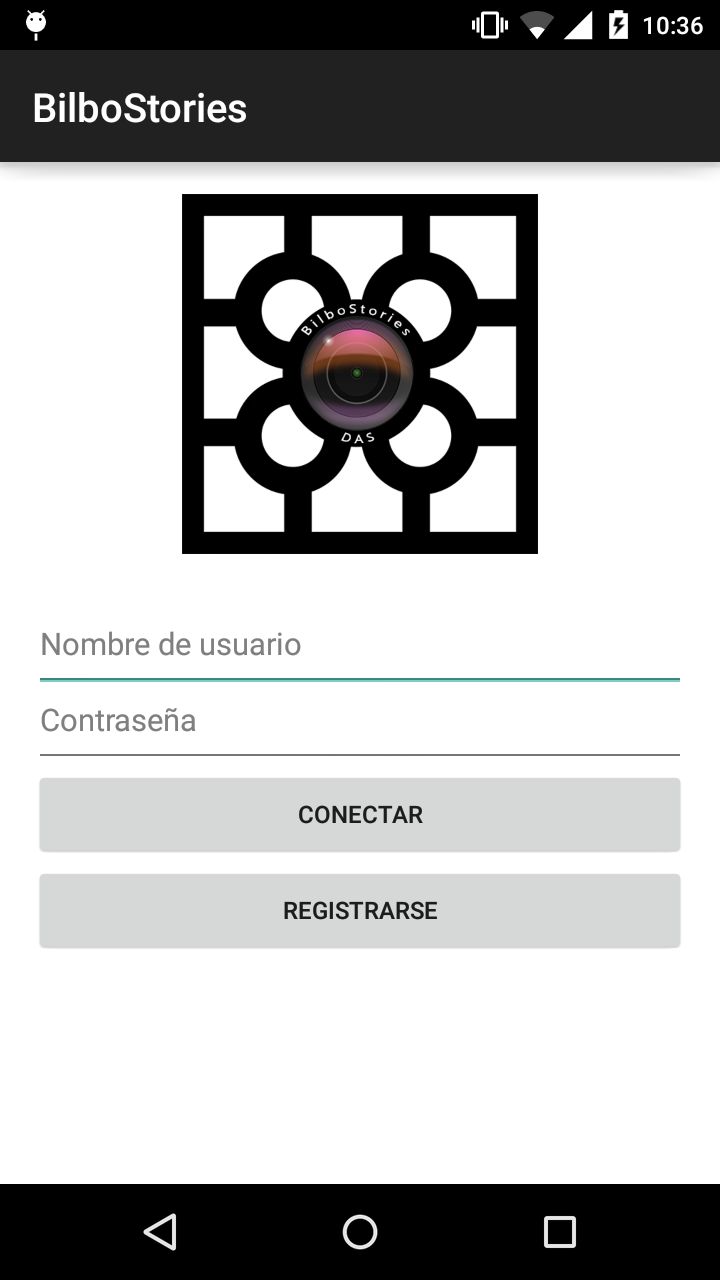
\includegraphics[scale = 0.25 ]{img/0}
		\caption{Log In}
		\label{}
	\end{figure}
	
Para poder utilizar la aplicación debemos introducir en los campos correspondientes un nombre de usuario y una contraseña registrados y pulsar el botón Log In.
	
	\begin{figure}[hbtp]
		\centering
		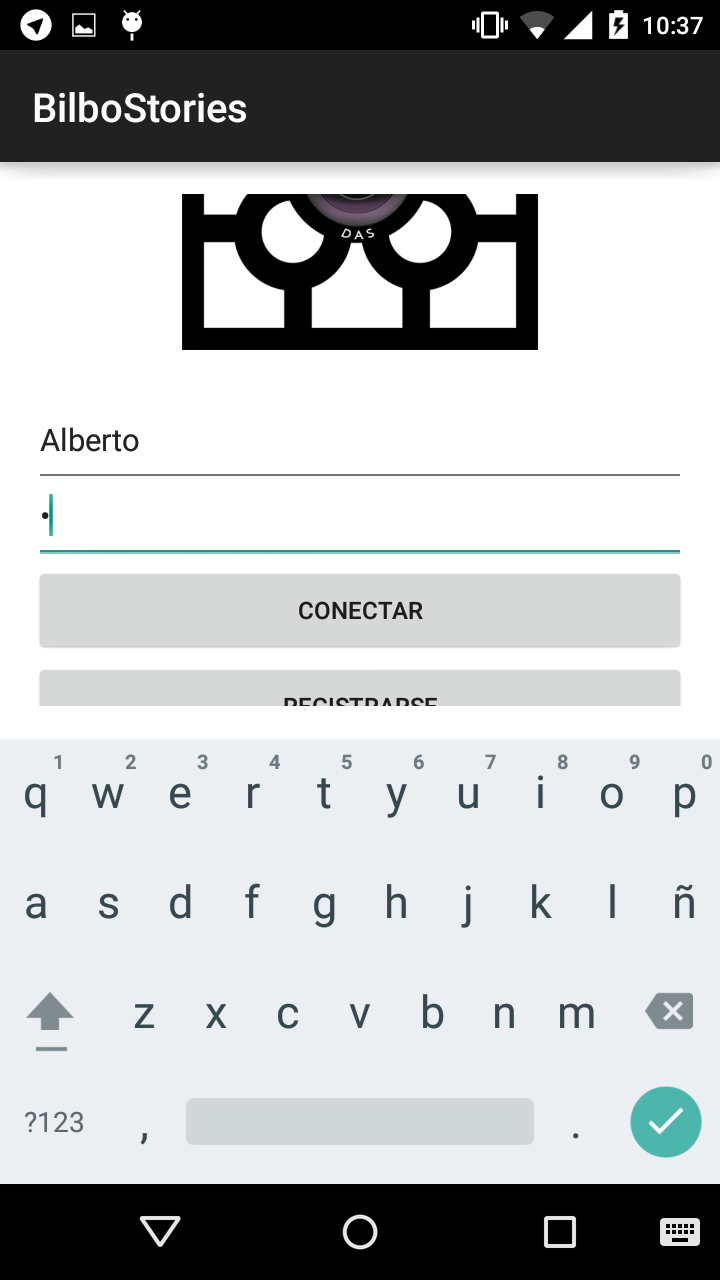
\includegraphics[scale = 0.25 ]{img/1}
		\caption{Log In}
		\label{}
	\end{figure}
	
	Si el usuario y contraseña son correctos se nos llevara automáticamente a la Pantalla principal, en caso contrario aparecerá un mensaje de error y tendremos que reintroducir los datos correctos o crear un nuevo usuario pulsando el botón Registrarse.
	
	\section[Registro]{Registro}
	\label{regis}
	
	Esta pantalla es la que nos permite crear un nuevo usuario para la aplicación. 
	
	\begin{figure}[hbtp]
		\centering
		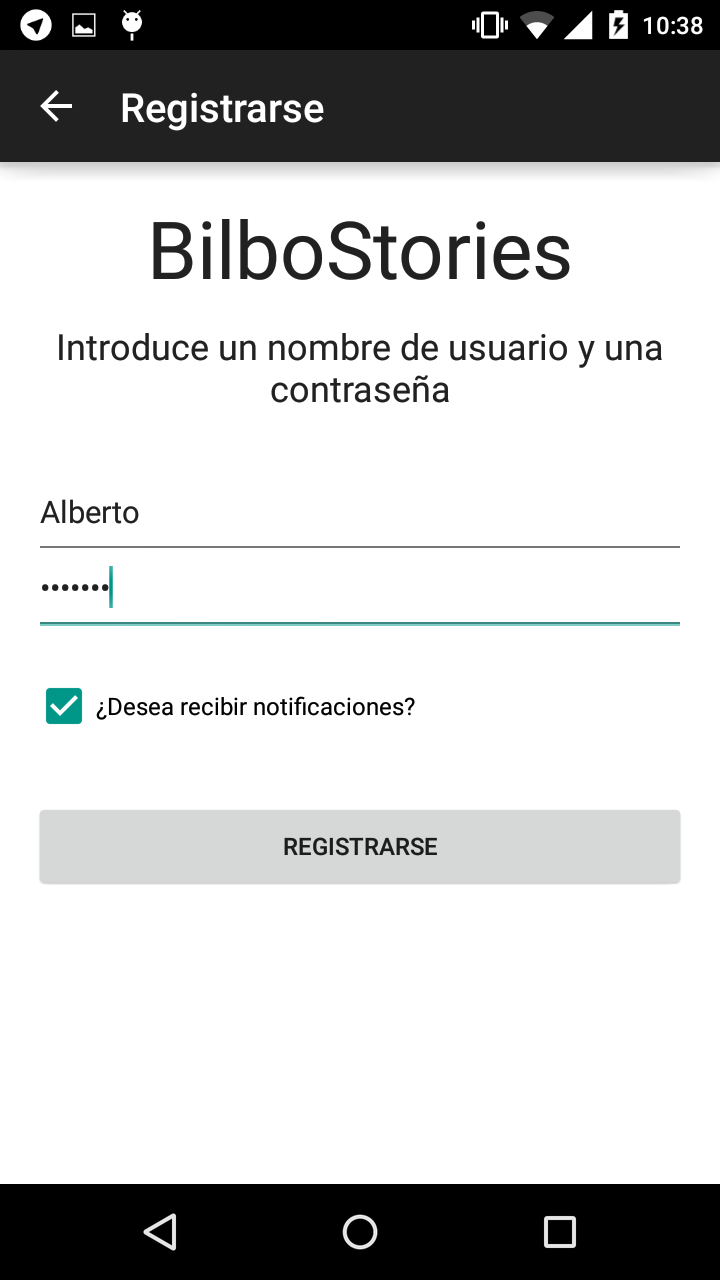
\includegraphics[scale = 0.25 ]{img/2}
		\caption{Registro}
		\label{p14}
	\end{figure}
Cuenta con dos campos donde insertar texto (nombre de usuario y contraseña), un checkbox donde indicar si se desean recibir avisos sobre nuevas publicaciones y dos botones, el primero de ellos para registrar un usuario con los datos introducidos y otro para cancelar el proceso.

Tras introducir los datos y pulsar el botón registrarse retornamos a la pantalla de Log In.
	
	\section[Pantalla Principal]{Pantalla Principal}
	\label{inPrin}
	
	Esta es la pantalla principal de la aplicación, cuenta con un menú lateral que nos permite acceder a las distintas funcionalidades de la aplicación:
	
	\begin{itemize}
		\item Listar las ultimas historias
		\item Listar las etiquetas que estamos empleando para categorizar las historias
		\item Listar las mejores historias
		\item Modificar datos de la cuenta que estamos utilizando
		\item Cerrar sesión
	\end{itemize}
	
	\begin{figure}[hbtp]
		\centering
		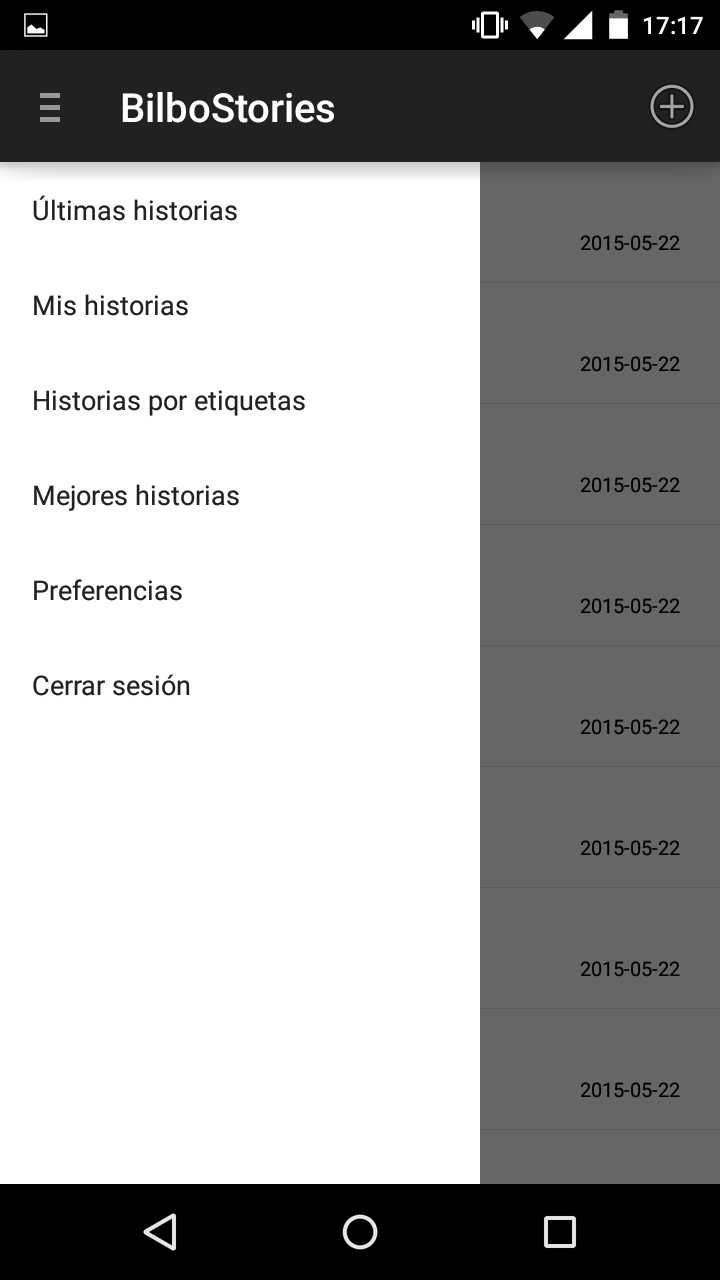
\includegraphics[scale = 0.25 ]{img/3}
		\caption{Pantalla Principal}
		\label{p1}
	\end{figure}
	
	El menú es accesible desde cualquiera de las funcionalidades de listado y la de modificación de preferencias.
	
	\section[Ultimas Historias]{Ultimas Historias}
	
	Esta funcionalidad es la encargada de mostrarnos las historias que han sido creadas o modificadas más recientemente.
	
	\begin{figure}[hbtp]
		\centering
		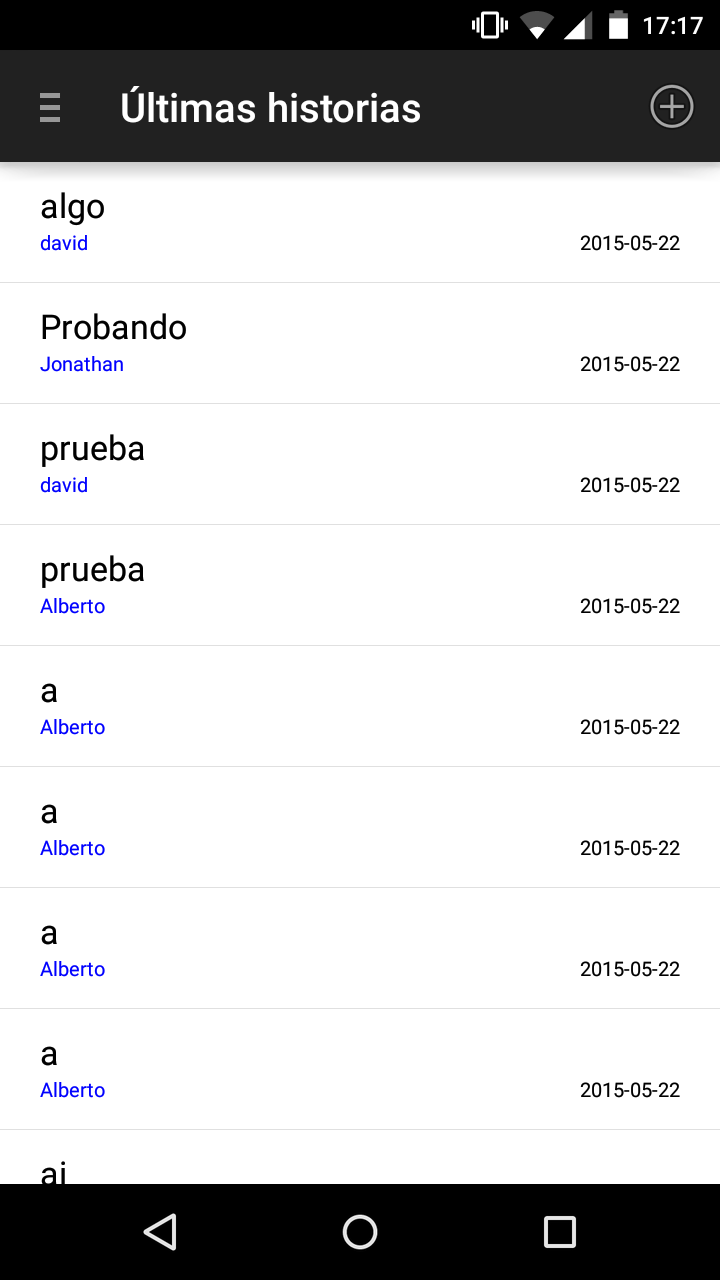
\includegraphics[scale = 0.25 ]{img/4}
		\caption{Ultimas Historias}
		\label{p1}
	\end{figure}
	
	Si pulsamos alguna de las historias de la lista se abrirá una nueva ventana que muestra en detalle la historia seleccionada.
	
	\section[Mis Historias]{Mis Historias}
	Esta funcionalidad es la encargada de mostrarnos las historias que han sido por el usuario con el que hemos iniciado la aplicación.
	
	\begin{figure}[hbtp]
		\centering
		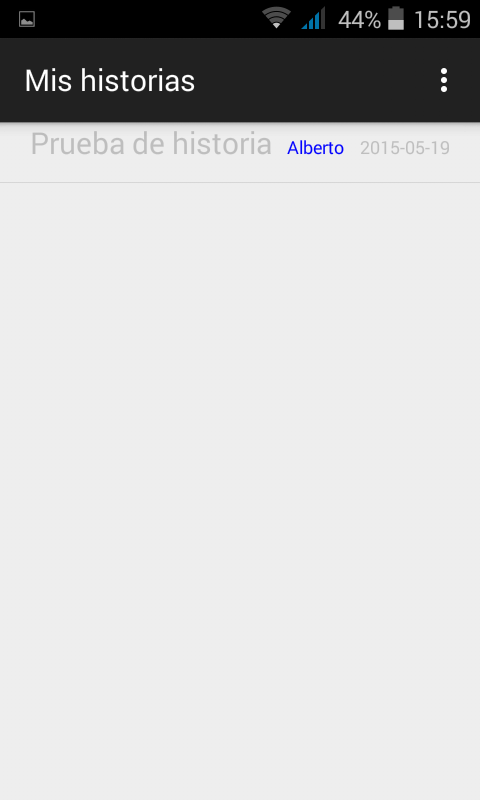
\includegraphics[scale = 0.25 ]{img/5}
		\caption{Mis Historias}
		\label{p1}
	\end{figure}
	
	Si pulsamos alguna de las historias de la lista se abrirá una nueva ventana que muestra en detalle la historia seleccionada.
	
	\section[Por Etiquetas]{Por Etiquetas}
	
	Esta funcionalidad es la encargada de mostrarnos la lista de etiquetas encargadas para categorizar las historias disponibles, junto al nombre se muestra el número de historias que tienen esa etiqueta asignada.
	
	\begin{figure}[hbtp]
		\centering
		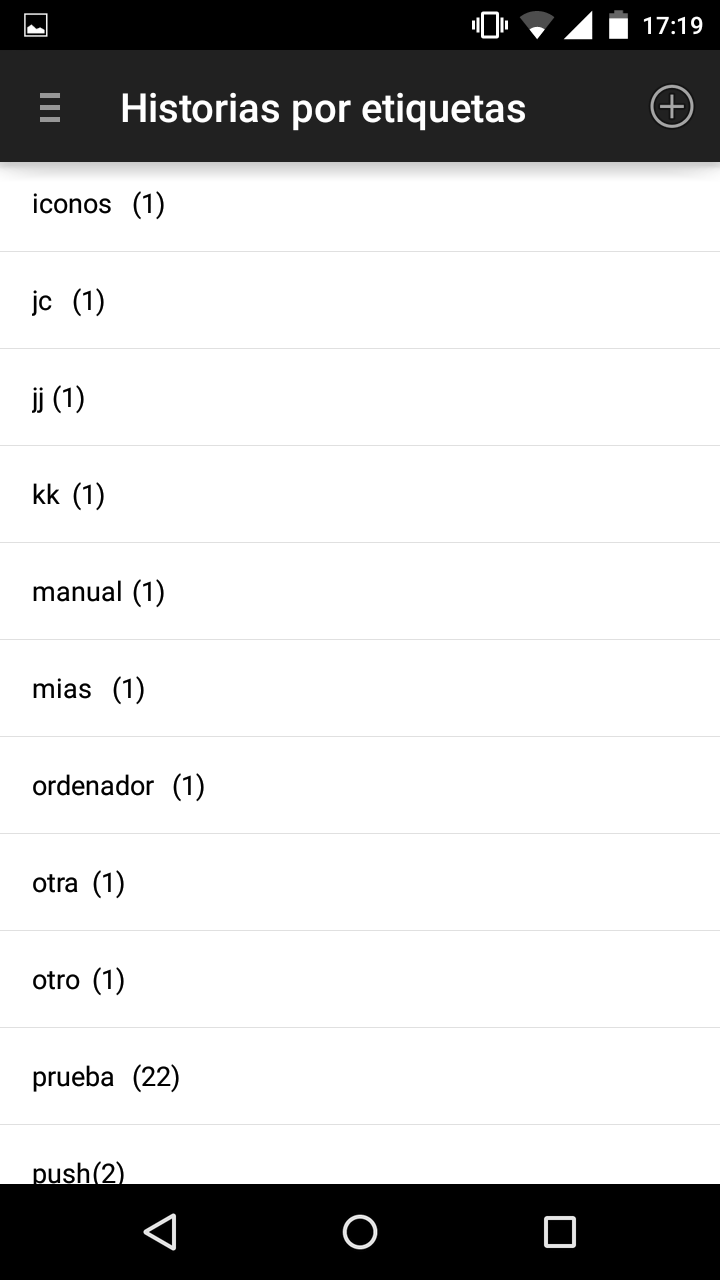
\includegraphics[scale = 0.25 ]{img/6}
		\caption{Por Etiquetas}
		\label{p1}
	\end{figure}
	
	Si pulsamos una de las etiquetas se nos muestra una lista con las historias que tienen la etiqueta pulsada asignada.
	
	\begin{figure}[hbtp]
		\centering
		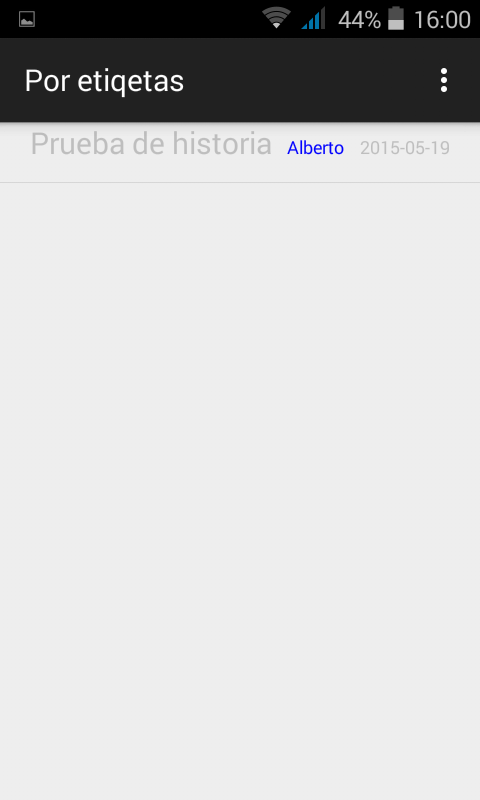
\includegraphics[scale = 0.25 ]{img/7}
		\caption{Por Etiquetas}
		\label{p1}
	\end{figure}
	
	\section[Mejores]{Mejores}
	
	\section[Preferencias]{Preferencias}
	
	Esta funcionalidad nos permite modificar la contraseña para el usuario con el que hemos iniciado la aplicación y modificar la opción de recibir avisos sobre nuevas publicaciones.
	
	\begin{figure}[hbtp]
		\centering
		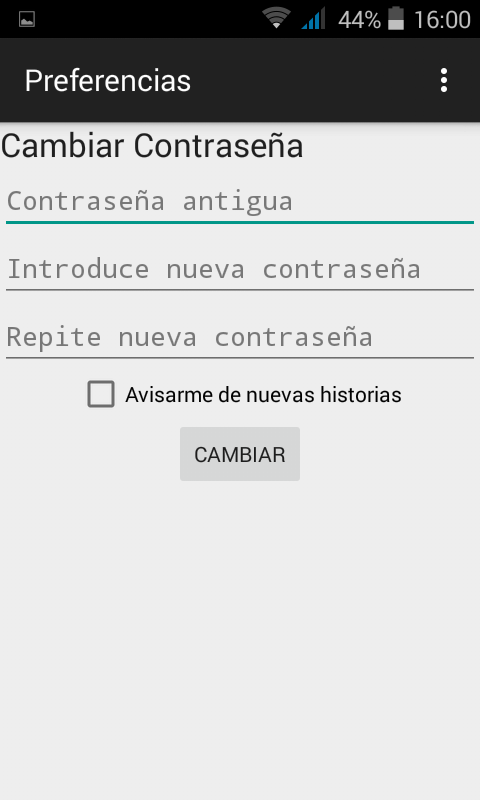
\includegraphics[scale = 0.25 ]{img/9}
		\caption{Preferencias}
		\label{p1}
	\end{figure}
	
	Para ello debemos introducir la antigua contraseñan, dos veces la nueva contraseña, si se desea seleccionar el checkbox de avisos y pulsar el botón cambiar.
	
	\section[Cerrar Sesión]{Cerrar Sesión}
	Esta funcionalidad nos permite hacer log out de la aplicación y nos lleva a la pantalla de log in para poder iniciar la aplicación con otro usuario . 
	
\end{document}